\chapter{Introduction}

%What are SARs and why are they important?
%Why is the theory important? 
The species--area relationship (SAR) is one of the oldest fundamental ecological laws \cite{GooriahLeanaD2019Sedt}. SARs describe the relationship between community diversity and habitat area. The observation that species richness increases with sampling area, a positive SAR, has been observed for a broad range of faunal \cite{ricklefs1999roles} \cite{lomolino1982species} \cite{eadie1986lakes} and floral groups \cite{zacharias1990species} \cite{price2011phylogenetic}. The ubiquitous nature of positive SARs has been used to inform conservation practises in natural \cite{haila2002conceptual} \cite{samson1980island} and urban environments \cite{davis1978urban}. Whilst a large number of studies have examined macro-organism SARs, relatively little is known about the spatial scaling of microbial biodiversity. \\

%Why is it important?
{\texorpdfstring
\noindent UUnderstanding the factors that regulate microbial community structure is important as they play a vital role in biogeochemical cycling and ecosystem functioning \cite{griffiths2011bacterial}. Despite bacteria and fungi representing major contributors to soil biodiversity and processes, little is known about below-ground regulators of biodiversity \cite{griffiths2011bacterial} \cite{li2020island}. This is especially challenging as few terrestrial environments present insular habitats for microbial community dynamics to be easily studied. Microorganisms also play a metabolically active role in polar regions previously believed to be abiotic \cite{stibal2020glacial}. Rapid climate change is leading to the exposure of soils dominant in high-latitude carbon \cite{bradley2017microbial}. As these soils are colonised by microbial communities, biogeochemical transformations release CO\textsubscript{2}, CH\textsubscript{4} and N\textsubscript{2}O. Understanding the mechanisms that drive microbial colonisation of polar environments can help produce accurate models of greenhouse gas release \cite{malard2018microbial}.} \\

%History of Microbial SARs
\noindent Debate around the applicability of SARs to microbial systems stems from the assumption that they are limited only by niche-filtering, as articulated by Bass-Becking: `\textit{Everything is everywhere}, but, \textit{the environment selects}' \cite{baas1934geobiologie}. This classic tenet of microbiology assumes that the abundance, short generation times and small size of microorganisms gives them an almost cosmopolitan distribution \cite{GreenJessica2006Ssom}. High abundances increase the probability of transport between environments via an accidental vector. Small size also increases the likelihood of passive transport via air or water, leading to high dispersal rates \cite{GreenJessica2006Ssom}. Uninhibited dispersal may also be facilitated by dormancy as a biogeographical response \cite{LoceyKennethJ2010Stbw}. \\

%The species-area relationship power-law model
\noindent One of the most commonly used tools in biogeography is the power-law model:

\begin{equation}
S=cA^{z}
\end{equation}\\

\noindent Where \textit{S} is species richness as a function of area (\textit{A}), \textit{c} is a constant specific to that taxa/habitat and the \textit{z} exponent is the slope of the line associating area and species richness \cite{darcy2018island}. \textit{z} typically falls in the range of 0.1 to 0.3 for continuous habitats and 0.25 to 0.35 for insular habitats \cite{GreenJessica2006Ssom}. Microbial \textit{z} values are typically well below those seen in macro-organisms (z < 0.1), supporting the idea of cosmopolitan distribution \cite{GreenJessica2006Ssom}. \\

%Problems with Microbial SARs
%Distribution maps define the annual or seasonal spatial distributions of functional groups and life stages, for simulating spatial patterns of predator-prey interactions
\noindent One of the limitations for microbial biogeography has been in quantifying taxa, given that many cannot be accurately identified using morphological techniques \cite{GreenJessica2006Ssom}. Commonly, microbial biogeography is concerned with taxa-area relationships (TARs), rather than SARs as microbial diversity is quantified in operational taxonomic groups (OTUs). Deciduous leaves as 'island' habitats for aquatic fungi found morphospecies-based diversity increased with leaf area, but next generation sequencing did not. \cite{duarte2017taxa}. With recent advances in molecular approaches such as single-celled sequencing, the genomes of previously uncultivated bacterial taxa are filling in the phylogenetic tree providing a higher resolution picture of microbial community structure \cite{lasken2014recent}. Limited data on temporal and spatial microbial distributions has led to a lack of detailed distribution maps. Distribution maps allow us to estimate the true number of taxa in a given environment when total counts are not available, without which estimated \textit{z} values may be artificially low \cite{GreenJessica2006Ssom}.\\


\noindent The mechanisms driving island SARs have been of particular interest to ecologists since the 1800s \cite{macdonald2018theory}. Islands are considered important paradigms for fragmented habitats as well as larger geographic regions \cite{simberloff1974equilibrium}. Their insular nature allows for ecological processes and patterns to be investigated in a simplified and relatively closed system. \\

%The general theory of island biogeography
%What is the theory about?

\begin{figure}[htp]

\centering
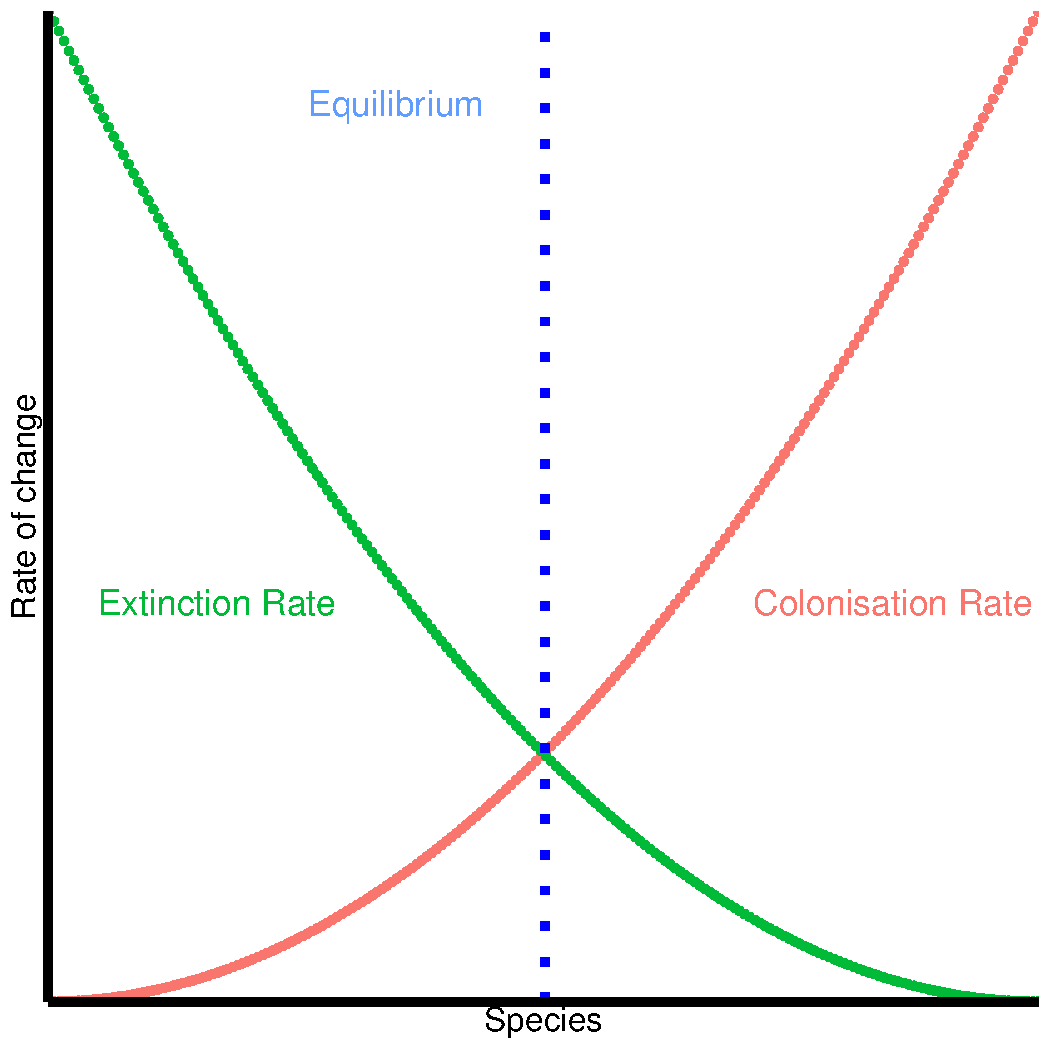
\includegraphics[width=.5\textwidth]{ColonisationDynamicEquilibrium.pdf}\hfill

\caption{Colonisation-Extinction Dynamic Equilibrium}
\label{fig:figure1}

\end{figure}

\noindent MacArthur and Wilson's Theory of Island Biogeography \cite{MacArthurRobertH1967Ttoi} is one of the most widely accepted island SAR theories. Explains the maintenance of biodiversity on islands through the stochastic processes of colonisation and extinction. The rates of these processes are determined by island area and isolation from the mainland. Islands that are nearer to source populations will experience a higher rate of immigration. This in turn can produce a rescue effect leading to decreased extinction rates \cite{brown1977turnover}. Larger islands will receive more immigrants as species actively target larger habitats with more resources, or will be more likely to immigrate randomly due to island size. A larger population is also less susceptible to inbreeding depressions and random extinction \cite{macdonald2018theory}. This results in higher species richness at the point of balance between immigration and extinction rates (i.e. the colonisation-extinction dynamic equilibrium, Figure 1.1) for larger, less isolated islands. \\

%What other mechanisms can drive patterns of biogeography?
\noindent It has been suggested that the stochastic significance of area in predicting species richness has been overplayed, to the exclusion of deterministic mechanisms such as interspecific relationships, biotic and abiotic factors \cite{abbott1974numbers}. This is due to empirical evidence suggesting that smaller islands do not always follow the positive SAR pattern  \cite{triantis2006re} \cite{sfenthourakis2009habitat}. MacArthur and Wilson noted that archipelagos showed unusual SARs, with smaller island species-richness varying independently of size \cite{MacArthurRobertH1967Ttoi}. It appears when smaller habitats within a broad range of spatial scales are assessed, both deterministic and stochastic patterns can emerge \cite{lomolino2001towards}. This exception to MacArthur and Wilson's putative ecological law has been dubbed the small-island effect (SIE). \\

%Explainations of the SIE
\noindent Several hypotheses have been offered to explain the SIE. The 'subsidized island biogeography' hypothesis suggests that smaller islands have a greater edge to interior ratio, thus receive a greater amount of nutrients per unit area \cite{barrett2003small} \cite{anderson2001subsidized}. Secondly, extinction rates on islands may operate independently of area due to their environmental instability and high temporal turnover, where major episodic disturbances periodically wipe out colonising species \cite{MacArthurRobertH1967Ttoi}. Thirdly, the 'habitat hypothesis' suggests that diversity is limited on smaller islands, compared to larger islands \cite{triantis2008evolutionary}. However, the environmental instability and habitat hypotheses contradict empirical data that indicate small islands have unusually high numbers of species. The Habitat--Diversity Hypothesis addresses the SIE phenomena by stating that as observation area increases we encounter a greater range of habitats \cite{EdwardF.Connor1979TSaB}. Therefore, the theory predicts that species richness should increase with habitat diversity, which varies independently of area \cite{macdonald2018theory}.  \\

%Chisholm et al model and research
\begin{figure}[htp]

\centering
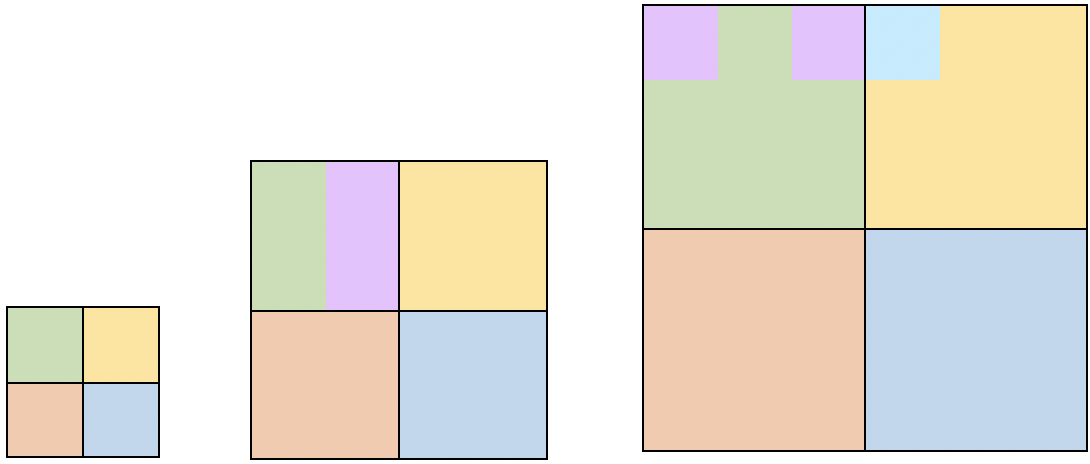
\includegraphics[width=.5\textwidth]{LowImIslands.png}\hfill

\caption{A graphical representation of a simulation (using the Classic Model, see Methods) of three islands of varying size, with the same number of niches (\textit{K}=4) and \textbf{low immigration rate} (\textit{m\textsubscript{0}} = 0.03). Each of the three main squares represents an island. Each smaller square represents an individual niche. Each unique colour patch within a niche represents a unique species. The smallest island has one species her niche, the medium size island has four individuals per niche and the largest island has nine individuals per niche. Species richness on the smallest island is \textbf{4}, on the medium island is \textbf{5} and the large island is \textbf{6}}
\label{fig:figure2}

\end{figure}

\begin{figure}[htp]

\centering
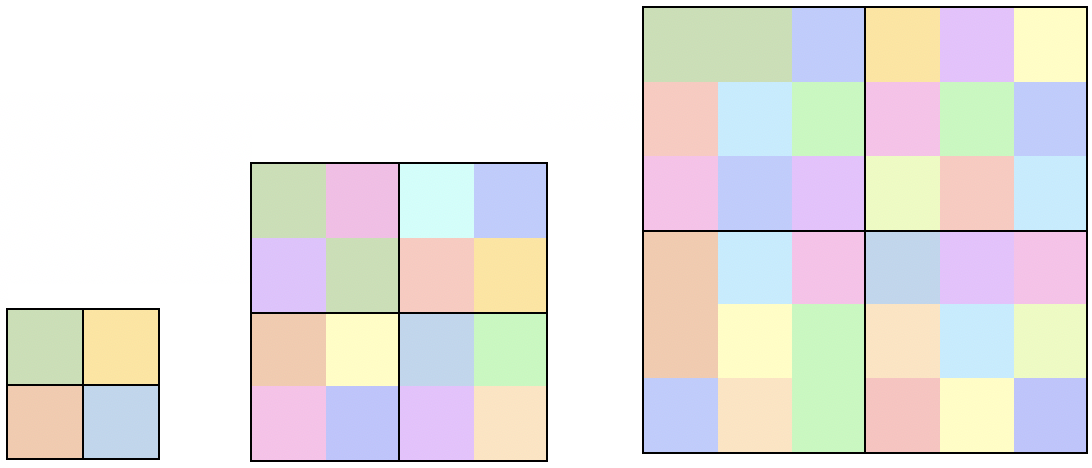
\includegraphics[width=.5\textwidth]{HighImIslands.png}\hfill


\caption{A graphical representation of a simulation (using the Classic Model, see Methods) of three islands of varying size, with the same number of niches (\textit{K}=4) and \textbf{high immigration rate} (\textit{m\textsubscript{0}} = 0.9). Each of the three main squares represents an island. Each smaller square represents an individual niche. Each unique colour patch within a niche represents a unique species. The smallest island has one species her niche, the medium size island has four individuals per niche and the largest island has nine individuals per niche. Species richness on the smallest island is \textbf{4}, on the medium island is \textbf{15} and the large island is \textbf{33}}
\label{fig:figure3}

\end{figure}

\noindent Chisholm \textit{et al.,} (2016) explain both deterministic and stochastic SARs in a unified theory. They posit that this pattern of species-richness is due to a transition from a niche-structured regime on smaller islands, to a colonisation-extinction regime on larger islands. The niche-structured regime is characteristic of deterministic theories like the Habitat--Diversity Hypothesis, where habitat structure and intra- and interspecific interactions determine species richness \cite{chase2011disentangling}. The colonisation-extinction regime is characteristic of stochastic mechanisms such as the Theory of Island Biogeography and ecological neutral theory, where richness is dictated by random colonisation and extinction events, as well as ecological drift \cite{hubbell2001unified}. Chisholm \textit{et al.,} hypothesise that species richness on all islands is maintained by these two mechanisms. They suggest that niche diversity increases slowly with area, whilst immigration rate increases quickly. Thus smaller islands are constrained by niche-structured regimes, until a critical area threshold where species richness is constrained by immigration. Figures 1.2 and 1.3 show the effect of immigration rate and area on species richness, where each 'island' is made up of four niches and the different coloured patches inside each niche represent a species unique to that niche. For islands with low immigration (Figure 1.2) or high immigration (Figure 1.3), small islands harbour the same number of species. Small islands where each niche can support only a small number of individuals will be constrained by those niches. Larger islands have less species at lower immigration rates and more species at higher immigration rates. They are less constrained by the number or size of their niches, and their species richness is dictated by random immigration and extinction events. \\

\noindent Chisholm \textit{et al.,} developed a parsimonious mechanistic model to test their hypotheses, and applied it to 100 archipelago datasets. Their results supported the prediction that critical area will be lower for species with higher motility and less isolated habitats. \\

%what do we know about the mechanisms driving microbial TARs? Deterministic niche regimes vs stochastic neutral regimes
\noindent Previous research indicates that microbial TARs may be controlled by either deterministic, environmental mechanisms, or stochastic, neutral processes \cite{StegenJamesC2012Sada}. Phylogenetic analysis of subsurface microbial communities showed related taxa utilised similar habitats, illustrating that environmental filtering determined community composition \cite{StegenJamesC2012Sada}. Niche filtering also had a greater influence in the most spatially and temporally varied environments \cite{StegenJamesC2012Sada}. The relative strength of these mechanisms has also been shown to vary with community functionality \cite{CarusoTancredi2011Sadp}. \\

\noindent Whilst both stochastic and deterministic processes are demonstrated for microbial communities, few studies discuss the transition of mechanisms across a spatial scale. An investigation of phytoplankton TARs in water bodies indicated that for the smallest spatial scales, niche relations determine OTU richness, before transitioning to an immigration dominated regime \cite{varbiro2017functional}. The SIE has also been seen in benthic diatoms where it is suggested stochastic variation in OTU richness is a function of the decreased stability of smaller habitats \cite{bolgovics2016species}. \\

%Aquatic Microbial TARs
\noindent Aquatic habitats are some of the most studied in microbial biogeography due to the availability of insular water bodies and their range of spatial scales. An investigation into bacterial diversity in aquatic tree holes found a \textit{z} value comparable to macro-organisms (\textit{z} = 0.26) \cite{bell2005larger}. Antarctic cryoconite holes have also exhibited positive TARs on glaciers where biomass influx was limited, illustrating the significance of immigration rate \cite{darcy2018island}. Positive associations between habitat area and microbial OTU richness have also been reported for habitats as diverse as lakes \cite{battes2019species}, membrane bioreactors \cite{van2006bacterial} \cite{van2005island} and vertebrate bodies \cite{godon2016vertebrate}.\\

%Terrestrial Microbial TARs
\noindent Previous investigations into ectomycorrhizal fungi communities within 'tree island' root systems showed that total OTU richness increased significantly with size, although distance effects vary \cite{glassman2017theory} \cite{peay2007strong}. An investigation into bacterial and fungal diversity in a group of land-bridge islands showed OTU richness for both groups was positively correlated with area, but these same patterns were driven by different mechanisms \cite{li2020island}. The bacterial TAR was a produce by differences in habitat quality with island area, and the fungal TAR was driven by within--island dispersal limitation. Laboratory based experiments have supported the presence of soil microbial TARs as well as the influence of resource availability on OTU richness \cite{delgado2018experimentally}. Country and continent-scale patterns of pathogen diversity have also been shown to be a function of area and isolation \cite{jean2016equilibrium} \cite{cashdan2014biogeography}. In both terrestrial and aquatic systems microbial communities exhibit significant TARs. The varying mechanisms underlying these TARs warrant further investigation. \\

\noindent In this project I apply three modified versions of the model presented by Chisholm \textit{et al.,}: \\

\noindent {$\cdot$ \textbf{Classic Model}: Where per capita immigration rate is proportional to habitat area (e.g. in the case of aerial and directed dispersal species immigrating into a two-dimensional habitat)} \\
\noindent {$\cdot$ \textbf{Perimeter Model}: Where per capita immigration is proportional to habitat perimeter (e.g. in the case of water dispersed species immigrating into a two-dimensional habitat) } \\
\noindent {$\cdot$ \textbf{Depth Model}: Where per capita immigration rate is proportional to depth (e.g. in the case of species dispersing into a volume via its surface into a three-dimensional habitat) }\\

\noindent These models are applied to bacterial, archaeal and micro-eukaryote insular spatial data with the aim of testing whether there is a biphasic microbial TAR, as well as investigating the impact of habitat type and taxonomic group on critical area of transition between the deterministic and stochastic regimes. 